
\section{Background}

Throughout Ontario, there is a clear desire to bring healthcare into the digital age by using software to improve access to medical information. The province intends to use a service-oriented architecture to allow for the development of components (i.e. IAPs) that distribute information between systems using a standard protocol known as the Health Information Access Layer (HIAL). HIAL will act as ``the broker and mediator for information exchange, ensuring that all [software] abide[s] by a common set of rules'' \cite{b1}. The intention of the government is to have a comprehensive and secure electronic health record, that may be accessed by HIAL-supporting software. This software may be developed by any vendor to support any patient or healthcare professional as the vendor sees fit. A systems diagram of Ontario's future eHealth infrastructure can be seen in figure~\ref{fig:eHealth1} below.


\begin{figure}[h]
  \centering
  \includegraphics[width=\linewidth]{diagramOntario.png}
  \captionsetup{format=hang}
  \caption[Ontario eHealth Systems View]{A systems view of Ontario's planned eHealth infrastructure, showing ``how EHR resources and services are integrated and deployed.'' \cite{b1}}
  \label{fig:eHealth1}
\end{figure}

In regards to software and hardware for EFRs, we talked to a number of paramedics about how technology can support and improve the care they provide. Currently, EFRs use software such as the system seen in Figures 1 to guide them through collecting data that may be important to a patients health. These systems are cumbersome, require time to fill, and are only as helpful as the information the paramedic manages to collect. Throughout our discussions, there was overwhelmingly interest in a system that could provide paramedics with patient medical history. We discovered that any information provided to a paramedic is helpful, and can greatly improve the quality and speed of care. In general, our findings can be summarized with the following quote from paramedic Matt Sartor:

\blockquote{Nursing homes carry [transfer documents] that contain updated information on [a patient] such as: medications, allergies and diagnosed disorders; including say if they [have] had a stroke, or have dementia, and what level of cognition or communication is normal for them. This kind of information gives us as paramedics a tipping point for how we assess our patients, or how we expect to communicate with them or have them do the same with us. [This information] would be very helpful for anyone we meet. Even if it's only [medication] history and allergies, we can decipher a lot from that. Even recent visits to hospital gives us a pattern of problems with a patient.

Currently the hospital can scan their card and get all prior hospital visits and diagnoses on discharges, but it's not available or compact enough for [paramedics] to get. If somehow our laptop forms, which we have to manually input all information we can attain, could get the aforementioned information, it would largely influence our practice.
}



\begin{figure}[h]
  \centering
  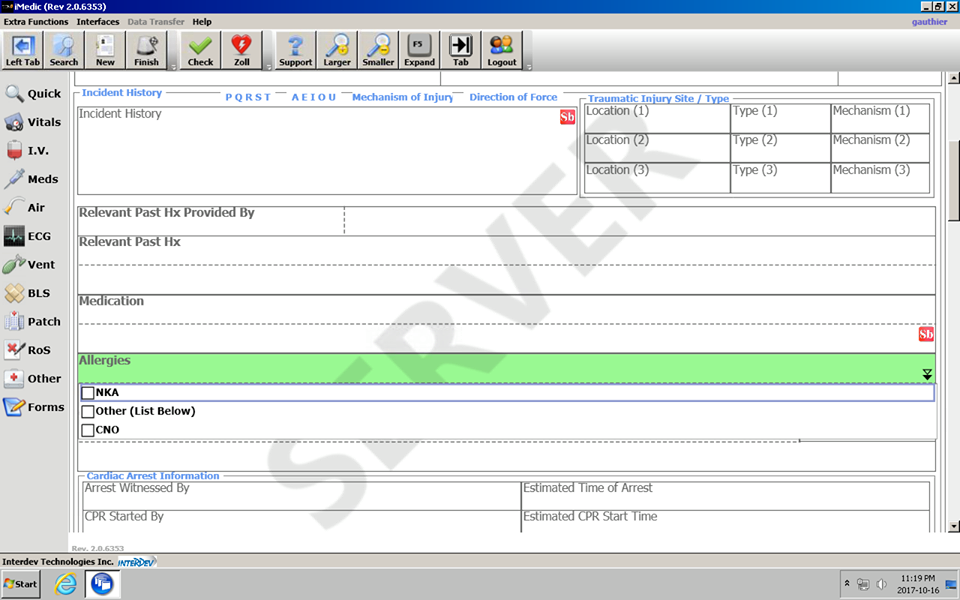
\includegraphics[width=\linewidth]{iMedic.png}
  \captionsetup{format=hang}
  \caption[Screenshot of iMedic Software]{A screenshot of the current software, iMedic, used by paramedics when responding to a call.}
  \label{fig:eHealth1}
\end{figure}


\iffalse

Throughout Ontario, there is a clear desire to bring healthcare into digital age by using software to improve access to medical information. The Ontario government has outlined the direction Ontario's digital health infrastructure will take in the future, employing a "service-oriented architecture" to distribute medical information.  The province intends to provide patients and healthcare professionals with information through a comprehensive and secure electronic health record stored on (central servers), and accessed through dedicated information portals. Information provided to professionals will be specific to the care they offer, ensuring a patients medical history is distilled into its most relevant components.


future electronic health records and consuming systems.

 using a set of protocols and rules to govern


, allowing components to be developed independently of each other.


ato provide patients and healthcare professionals with information relevant to them \cite{b1}. Specifically, a comprehensive and secure electronic health record will be distributed to dedicated information portals using a standard health information access layer (HIAL) protocol  stored on (central servers), and accessed through dedicated information portals. Information provided to professionals will be specific to the care they offer, ensuring a patients medical history is distilled into its most relevant components.


With our objectives in mind, we have talked to a number of paramedics about our project, and their response was overwhelmingly positive. There is general consensus among the paramedics we have talked to that medical history is vital to their job, and that any information about a patient can help them provide more appropriate care. Paramedics also expressed support for a software and hardware system that can help track patient vitals, and record any relevant information information. Our discussions with paramedics can be summarized by the following quote from paramedic Matt Sartor:

\blockquote{Nursing homes carry [transfer documents] that contain updated information on [a patient] such as: medications, allergies and diagnosed disorders; including say if they [have] had a stroke, or have dementia, and what level of cognition or communication is normal for them. This kind of information gives us as paramedics a tipping point for how we assess our patients, or how we expect to communicate with them or have them do the same with us. [This information] would be very helpful for anyone we meet. Even if it's only [medication] history and allergies, we can decipher a lot from that. Even recent visits to hospital gives us a pattern of problems with a patient.

Currently the hospital can scan their card and get all prior hospital visits and diagnoses on discharges, but it's not available or compact enough for [paramedics] to get. If somehow our laptop forms, which we have to manually input all information we can attain, could get the aforementioned information it would largely influence our practice.
}



\fi


We came across a document made in 2003 that outlined the possibility of implementing a medical information system through a “smart card”. The paper outlines how a “smart card” would implement QRF technology, that when scanned, would bring up the patients medical history. However, this method has the medical history actually being stored in the card itself. We want to design a database and use, lets say a health card, as just an ID, rather than the storage of the data itself.
Before developing a database, and the app to access the database, we first need to determine what relevant information we would need to be stored in the database. When talking to a paramedic, he gave this as a response to what information would be helpful:
Nursing homes carry a transfer document that (should) contain updated information on them such as: medications, allergies, and diagnosed disorders, including say if they had a stroke or have dementia, what level of cognition or communication is normal for them. This kind of information gives us as paramedics a tipping point for how we assess our patients or how we expect to communicate with them or have them do the same with us. That would be very helpful for anyone we meet. Even if it's only medical history and allergies, we can decipher a lot from that. Even recent visits to hospital gives us a pattern of problems with a patient. Currently the hospital can scan their card and get all prior hospital visits and diagnoses on discharges, but it's not available or compact enough for us to get. If somehow our laptop forms, which we have to manually input all information we can attain could get the aforementioned information it would largely influence our practice. Currently there are 2-3 different documenting systems in use in Ontario. So no unfortunately it's not standardized, that being said, neither is the hospital retrieval software, so an external device and software would help to standardize at least the ohip card aspect of retrieval.
We are creating the system based off the fact that we have acquired all the information, so we are focusing on the storing and displaying of the data, rather than the acquisition of it. Therefore, we need to decide how to effectively display and store the data.
